\input{__header__}

\begin{document}
\paragraph{О-08}
Законы геометрической оптики. Дифракция света. Принцип Гюйгенса-Френеля. Метод зон Френеля. Классификация дифракционных явлений. Дифракция Фраунгофера на длинной прямоугольной щели: схема наблюдения, влияние ширины щели на дифракционную картину, условия наблюдения дифракции.\\

\textbf{Законы геометрической оптики}
Закон прямолинейного распространения света: в оптически однородной среде свет распространяется прямолинейно.\\
Закон отражения света: падающий и отраженный лучи, а также перпендикуляр к границе раздела двух сред, восстановленный в точке падения луча, лежат в одной плоскости (плоскость падения). Угол отражения γ равен углу падения α.\\
Закон преломления света: падающий и преломленный лучи, а также перпендикуляр к границе раздела двух сред, восстановленный в точке падения луча, лежат в одной плоскости. Отношение синуса угла падения α к синусу угла преломления β есть величина, постоянная для двух данных сред: 
$$\frac{\sin \alpha}{\sin \beta} = n$$

\textbf{Принцип Гюйгенса-Френеля. }\\

\begin{figure}[h]
\begin{center}
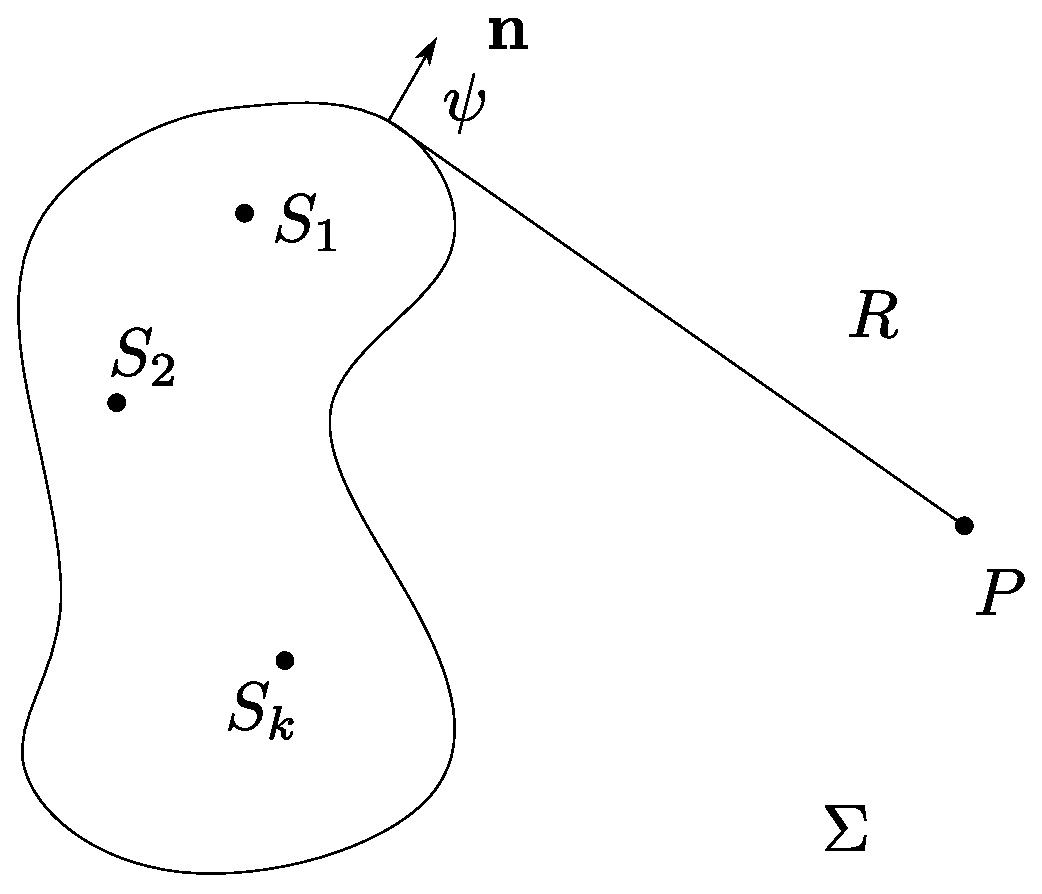
\includegraphics[width=0.5\linewidth]{img/o-08_1.eps}
\end{center}
\end{figure}

1. Если окружить систему когерентных источников произвольной замкнутой поверхностью $\Sigma$, то каждую точку этой поверхности можно считать источником вторичных когерентных сферических волн, распространяющихся по всем направлениям. Амплитуда этих волн на поверхности находится как суперпозиция волн, идущих от первичных источников. Световое поле в любой точке вне этой поверхности можно рассчитывать как суперпозицию всех вторичных волн. 
2. Если часть этой поверхности закрыта непрозрачным экраном, то учитывать нужно только волны, идущие от открытых частей поверхности.\\

Обе эти части принципа объединяет дифракционный интеграл Релея:
$$E(P) = \frac{1}{i\lambda}\iint\limits_{\Sigma'} \widetilde K(\psi) E(Q)\frac{e^{ikR}}{R}d\sigma,$$
где $\Sigma'$ - открытая часть поверхности $\Sigma$, $Q$ - точка на $\Sigma'$, $E(Q)\frac{e^{ikR}}{R}$ - сферическая волна, идущая от этой точки 


\textbf{Метод зон Френеля}\\

\begin{figure}[h]
\begin{center}
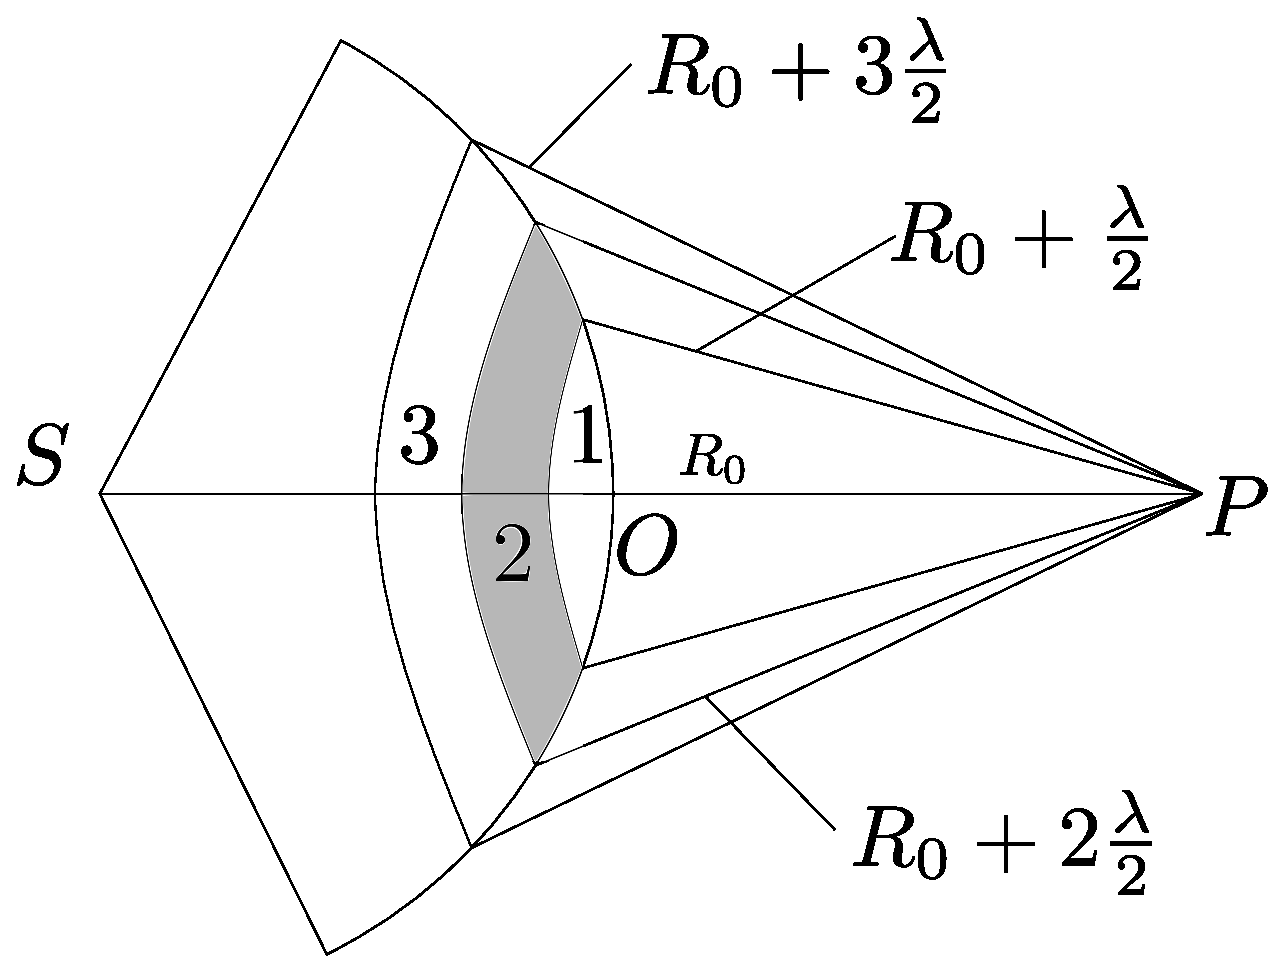
\includegraphics[width=0.5\linewidth]{img/o-08_2.eps}
\end{center}
\end{figure}

Суть наблюдаемого эффекта заключается в том, что при изменении в определенных пределах радиуса диафрагмы в точке $P$ наблюдается то светлое, то темное пятно. Для объяснения этого эффекта Френель предложил разбить вспомогательную поверхность на зоны. Первая зона Френеля представляет собой шапочку на сфере, граница которой отстоит от точки $P$ на расстояние $R_1 = R_0 + \frac{\lambda}{2}$, так что ей принадлежат все точки сферы в пределах $R_0 < R < R_0 + \frac{\lambda}{2}$. Все остальные зоны - пояса. Вторая зона задается условиями $R_0 + \frac{\lambda}{2} < R < R_0 + \frac{2\lambda}{2}$, ее внешняя граница удалена от точки наблюдения на расстояние $R_2 = R_0 + \frac{2\lambda}{2}$. Для $m$-той зоны:
$$R_{m-1} < R < R_m,$$
$$R_m = R_{m-1} + \frac{\lambda}{2} = R_0 + m\frac{\lambda}{2}$$
Используем формулу
$$E = E_0\left(K(R_{min}) e^{ik(R_{min} - R_0)} - K(R_{max})e^{ik(R_{max} - R_0)} \right)$$
В случае, если диафрагма открывает первую зону Френеля:
\begin{gather*}
R_{min} = R_0, \qquad R_{max} = R_0 + \frac{\lambda}{2} , \\
 e^{ik(R_{min} - R_0)} = 1, \qquad e^{ik(R_{max} - R_0)} = e^{ik\frac{\lambda}{2}} = e^{i\pi} = -1
\end{gather*}
Поле от первой зоны Френеля:
$$E^{(1)} = E_0(1 + K(R_1))$$
Аналогичные расчеты дадут для второй зоны Френеля:
$$E^{(1)} = - E_0(K(R_1) + K(R_2))$$
Для $m$ - той зоны:
\begin{gather*}
R_{min} = R_0 + (m - 1)\frac{\lambda}{2}, \qquad R_{max} = R_0 + m\lambda \\
e^{ik(R_{min} - R_0)} = e^{\frac{i(m-1)k\lambda}{2}} = e^{i(m-1)\pi} = (-1)^{m-1}, \qquad 
e^{ik(R_{max} - R_0)} = e^{ikm\frac{\lambda}{2}} = e^{im\pi} = (-1)^m\\
E^{(m)} = E_0\left((-1)^{m-1} K(R_{m-1}) - (-1)^m K(R_m)\right) = E_0(-1)^{m-1} (K(R_{m-1}) + K(R_m))
\end{gather*} 

\textbf{Классификация дифракционных явлений}\\

Если диафрагма закрыта, то понятно, что за ней нет никакой волны. Будем постепенно ее открывать. В точке наблюдения будет монотонно расти освещенность. В этой области ($m << 1$) на оси ничего интересного не происходит, но на экране наблюдаются кольца – дифракция уже есть и в этих условиях, она называется дифракцией Фраунгофера.
Мы уже устремили источник в бесконечность. Если $m << 1$,
то и точка наблюдения очень далеко ($b \rightarrow \infty$). На диафрагму падает почти параллельный пучок света, и за диафрагмой распространяются лучи параллельные лучи в различных направлениях. Поэтому дифракцию Фраунгофера еще называют дифракцией в параллельных лучах.\\
Так будет продолжаться до тех пор, пока число $m$ не станет равным единице – это максимум, соответствующий одной открытой зоне Френеля. Далее последует минимум с почти нулевой интенсивностью (две открытые зоны), и затем максимумы, уменьшаясь по интенсивности, будут чередоваться с минимумами, которые все больше и больше будут отличаться от нуля. Дифракция в условиях, когда число $m$ равняется нескольким единицам, называется дифракцией Френеля.
Наконец, при дальнейшем увеличении радиуса диафрагмы интенсивность становится равной интенсивности в отсутствие преград, лучи распространяются прямолинейно, так что при $m >> 1$ мы переходим в область геометрической
оптики.\\

\textbf{Дифракция Фраунгофера на длинной прямоугольной щели: схема наблюдения, влияние ширины щели на дифракционную картину, условия наблюдения дифракции.}\\

\begin{figure}[h]
\begin{center}
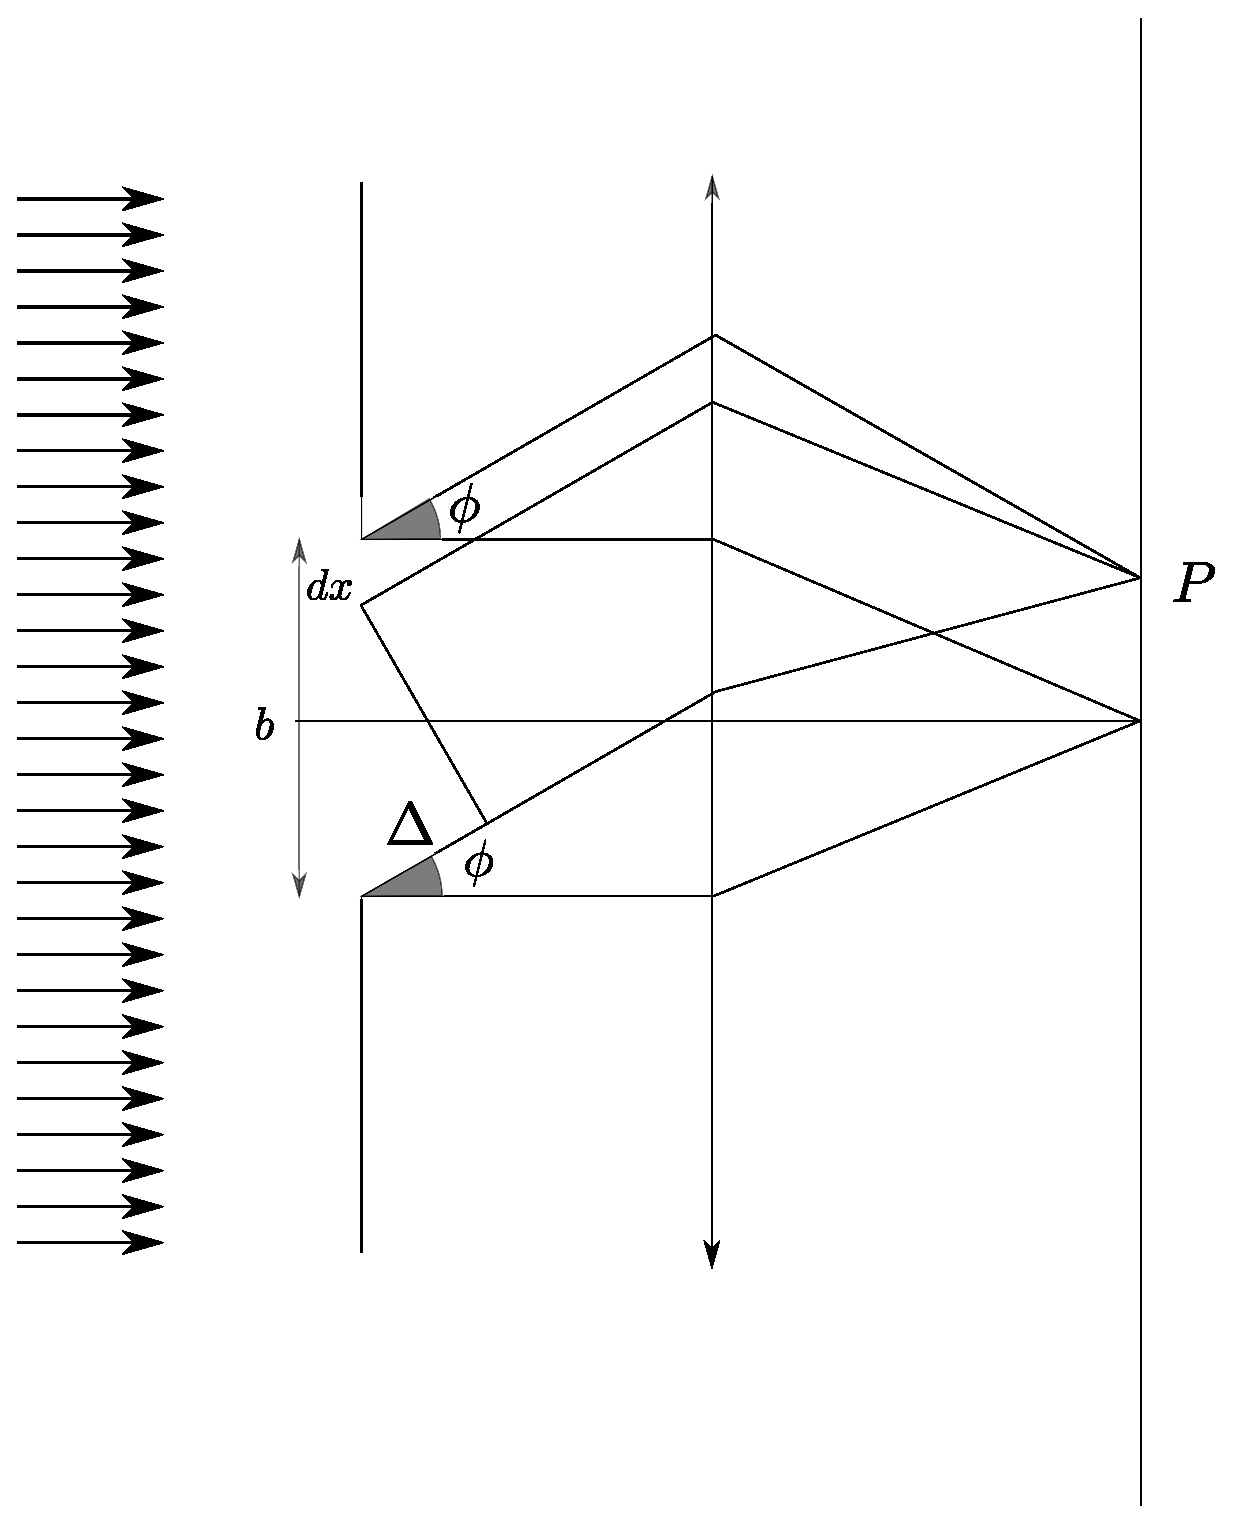
\includegraphics[width=0.5\linewidth]{img/o-08_3.eps}
\end{center}
\end{figure}

Дифракция Фраунгофера, как уже говорилось, это дифракция в параллельных лучах. Параллельный пучок света падает нормально на плоский экран со щелью шириной $b$ – и то, и другое перпендикулярно плоскости рисунка. За щелью расположена линза Л, в фокальной плоскости которой находится экран Э. Параллельные лучи, идущие от разных полос щели, собираются в полосы на экране. Например, элемент рисунка $dx$ представляет бесконечно узкую полосу. Идущие от нее лучи, перпендикулярные плоскости щели, собираются в центральную полосу, а лучи, идущие под углом $\phi$ к нормали – в точку $P$, которая также представляет целую полосу (точнее, линию) экрана Э, перпендикулярную плоскости рисунка. Далее мы будем просто говорить «точка», имея в виду, что во всех плоскостях, параллельных плоскости рисунка, все происходит в точности так же.
От всех элементов щели $dx$ лучи расходятся по всем направлениям, но в отличие от дифракции Френеля их можно считать плоскими волнами. Фазы и амплитуды колебаний во всех точках щели одинаковы.
Линза обладает важным свойством – она не вносит дополнительной разности фаз в падающие на нее параллельные лучи, которые собираются в фокальной
плоскости. Однако у лучей, идущих от различных элементов щели есть оптическая разность хода. Оптическая разность хода между лучом, идущим из элемента $dx$, и лучом от нижней точки щели О под углом $\phi$ к нормали равна $\Delta = x\sin\phi$\\
Если ширина щели меньше длины волны, то ничего не видно, кроме нулевого максимума – дифракционной картины как таковой нет.
Чем шире щель, тем\\
1) ярче картина\\
2) меньше контрастность\\
3) уже линии\\
4) больше число максимумов\\.
\\
Перечислим условия, при которых можно наблюдать дифракцию.
Поперечный размер объекта $b$ должен быть больше длины волны, $b > \lambda$ , но не может быть и слишком большим, так как\\
1) необходимо выполнения условия пространственной (поперечной) когерентности $b<\rho_{\text{когер}}$ ,\\
2) должно выполняться условие временной (продольной) когерентности $b\sin\phi < \frac{\lambda^2}{\delta \lambda}$. В роли ширины спектра $\delta\lambda$ может выступать цветовое разрешение глаза\\
3) если значение $m_{max}$ велико, то картина теряет контрастность; при этом может еще быть наблюдаемой дифракция Френеля, либо вообще речь уже
идет о геометрической оптике.
\end{document} 
